%\RequirePackage{luatex85,shellesc}
\documentclass[english]{scrartcl}
\usepackage{geometry}
	\geometry{
		letterpaper,
%		includehead,
		includefoot,
%		showframe,
		left=20mm,
		right=15mm,
		top=20mm,
		bottom=10mm,
		}
\usepackage{lmodern}
\usepackage{babel}
\usepackage{amsmath,amsfonts,amssymb}
\usepackage{graphicx}
\usepackage{float} 
	\restylefloat{figure}
\usepackage[version=4,arrows=pgf-filled]{mhchem}
\usepackage{setspace}
	\onehalfspacing

\usepackage{enumitem}

\usepackage{siunitx}
	\DeclareSIUnit{\dpi}{dpi} %dots per inch

%\usepackage{microtype}
\usepackage[pdfencoding=auto,pdftitle={Better pictures with JEOL SEM},pdfauthor={Thomas Lenk}, pdfstartview=FitV]{hyperref}
\title{Manual for LabView software to improve workflow with JEOL SEM at University of Michigan}
\subtitle{Version 1.0}
\author{Lenk, Thomas}
\begin{document}
\maketitle
\section{Copyright}
MIT License

Copyright (c) 2018 Thomas Lenk

Permission is hereby granted, free of charge, to any person obtaining a copy of this software and associated documentation files (the "Software"), to deal in the Software without restriction, including without limitation the rights to use, copy, modify, merge, publish, distribute, sublicense, and/or sell copies of the Software, and to permit persons to whom the Software is furnished to do so, subject to the following conditions:

The above copyright notice and this permission notice shall be included in all copies or substantial portions of the Software.

THE SOFTWARE IS PROVIDED "AS IS", WITHOUT WARRANTY OF ANY KIND, EXPRESS OR IMPLIED, INCLUDING BUT NOT LIMITED TO THE WARRANTIES OF MERCHANTABILITY, FITNESS FOR A PARTICULAR PURPOSE AND NONINFRINGEMENT. IN NO EVENT SHALL THE AUTHORS OR COPYRIGHT HOLDERS BE LIABLE FOR ANY CLAIM, DAMAGES OR OTHER LIABILITY, WHETHER IN AN ACTION OF CONTRACT, TORT OR OTHERWISE, ARISING FROM, OUT OF OR IN CONNECTION WITH THE SOFTWARE OR THE USE OR OTHER DEALINGS IN THE SOFTWARE.
\section{About this software}
This software is intended to ease your work flow of taking pictures at the JEOL SEM and use them for whatever publication you need - poster, paper, weekly reports to your supervisor, thesis, ... .
For some of those publications, you have to have high quality pictures, e.g. for publications you want to have pictures with a resolution high enough that you can print them with \SI{300}{\dpi} and the image shall still be large enough to cover half the width of a letter paper or large enough to be visible on a poster. Although getting a high resolution picture using the SEM software is easy, getting it into a publishable format is not. The work flow I got introduced to is to take the pictures, send them to a report, export this report as a PowerPoint file and deal with it from there. The PowerPoint file includes some scale bar, but making it look nice and getting a good image file with the right resolution is cumbersome, due to PowerPoints flaws or my lack of skill with it.\footnote{I prefer \LaTeX\ to Microsoft Word and PowerPoint.}

Another possible way is to export the images with a black bar below the picture showing all the information you might want (you usually don't care about this information when publishing), but this bar can't be changed in size. Therefore it might be hard to be read after scaling it to fit on a poster or in a paper.

Therefore I decided to program a small piece of software that allows you to add a scale bar in the picture with a color, position and size you can determine. Therefore it should be easier for you to get the pictures you need.
\section{How to install this Software}
If you have a computer running Windows 7 or higher, you have some options:
\begin{itemize}
	\item Download LabView 2016 or later (no LabView NXG branch) to edit or execute the VI files
	\item Use the executable file without the installer if you have a LabView 2016 Runtime Environment already installed.
	\item Use the installer if you don't fulfill the other 2 options. It will install all the necessary files.
\end{itemize}
If you have a Mac, you can install LabView 2016 or above as well to run the VIs. %I might be able to create an executable file for MacOS as well. Please be aware that not all features (especially the detection of installed fonts) might work on MacOS. <- skiped due to lack of time and a Mac with LabView.
\section{How to use this Software}
\begin{enumerate}
	\item Make sure you know how to get sharp and nice pictures with the right amount of contrast and brightness.
	\item Set Photo resolution to a desired value - I prefer the 2560x1920 resolution, because you could print that to a sheet of paper of about 8.5 by 6.5 inches at \SI{300}{\dpi}, which should be large enough for all applications including posters. The time needed for one picture could be set to \SI{40}{\second}, which is a reasonable compromise between speed and quality. See \autoref{fig:manual_1} for a screenshot of the available options for resolution and time. You can open this window by right clicking on the photo button. See also \autoref{fig:manual_2} for the options mentioned below. To get to this menu, select image in the menu displayed in \autoref{fig:manual_1}.
	\item Set Image format to PNG - I think PNG is the way to go here, because it is easier to handle than TIFF files. Therefore, the software can only handle PNG files.
	\item Unselect the save as grey scale image and save text file in compatible mode (Shift-JIS) options.\footnote{Those will only make ruler information you add displayed in gray (hard to see) and the corresponding text file saved with an encoding harder to decode correctly (especially the Greek letter $\mu$ as in \si{\micro\metre} might be displayed wrong). I have tried to circumvent the decoding problems, you still might have some issues if you forget to unselect this option!}
	\item Set the directory in the auto save box to the right path. This path will determine where your image with the information bar from the JEOL software will be saved. \footnote{The directory in the snapshot box is for snapshots only. Nevertheless, it does not hurt to set it to a path of your choice just to be sure.}
	\item Collect images as usual. This will save a image with the information bar from JEOL software.
	\item In the data collection window, you can also export already taken images as a PNG. Choosing this option also exports the necessary text file.\footnote{That allows you to get an image version with the JEOL software bar and one without it. That also allows you to export previously taken images to process them with this software.}
	\item Place all your images and the corresponding text files in the same folder.
	\item Start the software:
	\begin{itemize}
		\item Select either one PNG or the corresponding TXT file. To do so, click on the folder symbol next to path to single file. Navigate to the folder where you saved your files, select the corresponding file and press the OK button.
		\item Press load image. A preview is displayed in the area on the left. Use the scroll bars to navigate to the area, where the information will be inserted (lower left corner per default).
		\item Adjust all settings:
			\begin{itemize}
				\item Font settings: With a click on the font window, you can select any fonts installed on your PC (Windows only). If the selected font is not available, your operating system will select another one (LabView default behavior). Font size is in pixel. Bold enables (green)/disables (grey,standard) a bold version of your selected font, where applicable. Standard values are Arial, 60, non bold.
				\item Color settings: Clicking on the color fields opens a control panel where you can select any color you like. Transparent is available for the background color only and can be selected on the upper right corner (small square with a capital letter T on white background). Usually either black or transparent background color with a white information color is a good choice.
				\item Spacing:
					Background:
					\begin{itemize}
						\item Use picture width: Enables (green)/disables (grey, standard) the usage of the whole width of the image to display the background bar.									\item Add box below image: Add box either in the image (grey, default) or below image (green).
						\item Extra width/height of background box: Adds extra space around the information by adding about half of the values entered here above, below, to the left, and to the right of the information boundary box, respectively. If set to 0, the background width and height are determined by the width and height of the information to be displayed and fit tight. Standard values: 30 for both.
						\item x and y. Those values allow you to shift the background and information to the right (x) and up (y).\footnote{If you add box below image is enabled, then those values shift everything to the right and down.} Standard values: 50.
					\end{itemize}
					Scalebar:
					\begin{itemize}
						\item Height of bar: Sets the height of the scale bar. Standard value: 50.
						\item Width scaling factor: Scales the width of the scale bar. So if image meta-data from TXT file contains the information for a \SI{10}{\micro\metre} scale bar, then a \SI{20}{\micro\metre} scale bar would be displayed if you select a factor of 2 here.\footnote{This allows you to display the same length of scale bar, even if you have taken images with different magnification. No unit conversion will be made, so a scaling factor of 10 with a scale bar information of \SI{100}{\nano\metre} will result in a \SI{1000}{\nano\metre} scale bar, not in a \SI{1}{\micro\metre} one!}
						\item Precision: If you select a width scaling factor different from one, you might get numbers that require more decimal digits. To display those, increase the Precision. Standard value: 0 (no decimal digits).
					\end{itemize}
			\end{itemize}
		\item Press create preview. Check if it fits.
		\item If you need to make changes: Change settings, press load image again, press create preview again.
		\item Press save to save a new PNG file in the same directory as the original file, file name will be edited\_ followed by the original file name. Example: ABC.png and edited\_ABC.png.
		\item If you want to batch convert all images in one folder (non recursive) with the same settings, make sure that there are no PNG files without corresponding TXT files in that folder, select the directory and press save all images. That might take a while, depending on your computer and the number of pictures you have selected.
	\end{itemize}
\end{enumerate}
\begin{figure}[htbp]
	\centering
	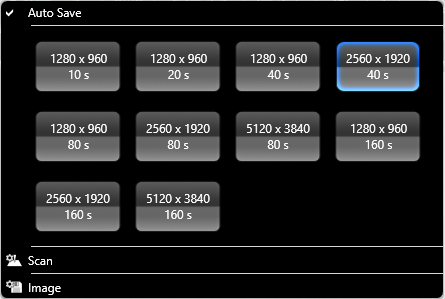
\includegraphics[width=.6\textwidth]{manual_1}
	\caption{Settings for resolution and capture time.}
	\label{fig:manual_1}
\end{figure}
\begin{figure}[htbp]
	\centering
	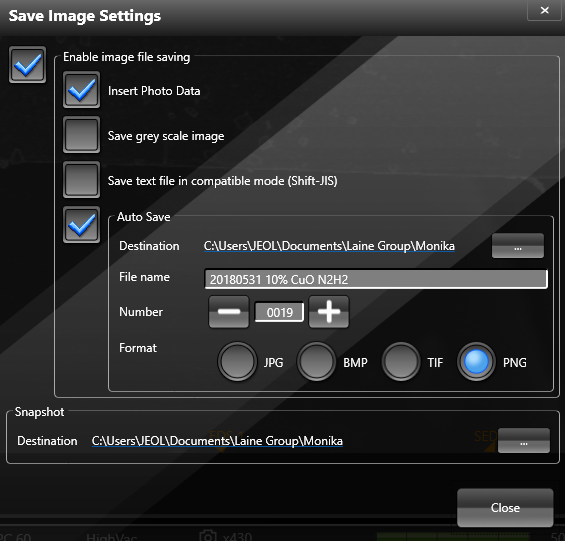
\includegraphics[width=.6\textwidth]{manual_2}
	\caption{Settings how to save a image.}
	\label{fig:manual_2}
\end{figure}

\section{How it works}
The TXT file holds all the necessary information needed to create the scale bar - The image resolution, the field of view and the scaling of the scale bar.
The software collects that data from the TXT file, does the necessary calculations for anything the user might want to do and draws the resulting rectangles and text to the right position in the image. The math is pretty straight forward.
\section*{Ideas}
\begin{itemize}
	\item Add multicore support (since all the information is predetermined, it is no problem to detect the number of cpu cores, divide all those images on those cores and let each core handle pictures. Right now, the software opens one picture at a time and on my laptop (i5 3317U, SSD) it takes quite some time to open the image, process the data, save the data while the CPU is used at \SI{25}{\percent} in this period. So expect long calculation times for larger file-sets, even on faster and more modern PCs. There is no progress bar (yet?), so don't lose your patience. Check the folder to see if there are new images showing up.
	\item Add a file where users can save/restore their preferences instead of setting them up each and every time. This could either be done using the LabView write/read an INI file or the read/write XML files.
\end{itemize}
\end{document}
